% File project.tex
%% Style files for ACL 2021
\documentclass[11pt,a4paper]{article}
\usepackage[hyperref]{acl2021}
\usepackage{times}
\usepackage{booktabs}
\usepackage{todonotes}
\usepackage{latexsym}
\usepackage{float}
\usepackage{caption}
\usepackage{subcaption}
\usepackage{enumitem}
\usepackage[normalem]{ulem}
\renewcommand{\UrlFont}{\ttfamily\small}
% This is not strictly necessary, and may be commented out,
% but it will improve the layout of the manuscript,
% and will typically save some space.
\usepackage{etoolbox} 
\AtBeginEnvironment{itemize}{\setlength\parskip{0pt}}
\AfterEndEnvironment{itemize}{\vspace*{-\dimexpr\parskip\relax}}
\usepackage{microtype}

% \titlespacing*{\section}
% {0pt}{0pt}{0pt}
% \titlespacing*{\subsection}
% {0pt}{0pt}{0pt}
% \titlespacing*{\subsubsection}
% {0pt}{0pt}{0pt}



\aclfinalcopy 

\newcommand\BibTeX{B\textsc{ib}\TeX}

\title{11-777 Spring 2021 Class Project}

\author{
  Andrew Singh\thanks{\hspace{4pt}Everyone Contributed Equally -- Alphabetical order} \hspace{2em} Ankit Ramchandani$^*$ \hspace{2em} Vashisth Parekh$^*$ \\
  \texttt{\{andrewsi, aramchan, vparekh\}@andrew.cmu.edu}
  }

\date{}

\begin{document}
\maketitle
\begin{abstract}
Template for 11-777 Reports using the ACL 2021 Style File 
\end{abstract}

\section{Introduction and Problem Definition (1-1.25 pages)}
\textbf{Thesis statement or Hypothesis we are aiming to prove}\\
``Our approach is better is not a hypothesis"

\clearpage
\section{Related Work and Background}
\label{sec:rel-work}
\subsection{ALFRED}
\label{ssec:alf}
Though ALFRED is a relatively new task, a multitude of approaches have recently been proposed that demonstrate improved performance over the baseline introduced in \cite{shridhar2020alfred}. The baseline model consists of a CNN to encode the visual input at each timestep, a bi-LSTM to encode the language directives, and a decoder LSTM to infer the action at each timestep while attending over the language encoding. \cite{corona2020modularity} used the same architecture as the baseline, except they maintained separate modules for each \emph{subgoal type} (e.g., GOTO, PICKUP). They then used a high-level controller to choose which module to execute at each step based on the language directives. \cite{singh2020moca} proposed a vision module for generating interaction masks and an action module for predicting actions, with the vision module first predicting the class of the object of interest and then generating the pixel-wise interaction mask given the predicted object class. \cite{Storks2021AreWT} addressed ALFRED's long action sequences by training the model to execute one subgoal at a time rather than all subgoals at once, and they address the agent's poor navigation performance by augmenting the agent's perception with additional viewing angles that are used for training an object detection module and for predicting the agent's orientation angle relative to the goal.

Unlike methods that learn a direct mapping from observations to actions end-to-end, \cite{Saha2021AMV} proposed a truly modular framework that is able to learn from unaligned or weakly aligned data as opposed to requiring expert demonstrations. Their mapping module includes a novel mapping scheme based on graph convolutional networks \cite{kipf2016semi} for improved navigation, and their language module leverages a pre-trained model to perform joint intent detection and slot filling on the language directives.

While the previously mentioned works improve upon the modeling approach proposed in the original ALFRED paper, \cite{Shridhar2020ALFWorldAT} also proposed a new environment to address the challenge of generalizing to unseen tasks. They aligned tasks in ALFRED with a purely textual environment, TextWorld \cite{Ct2018TextWorldAL}, allowing agents to first learn in an abstract setting in order to generalize better in the embodied setting. They additionally introduced a modular architecture to demonstrate the effectiveness of their ALFWorld environment, consisting of a state estimator that translates visual observations to text, an abstract text agent pre-trained in TextWorld that generates high-level actions from textual observations and a goal, and a controller that translates high-level actions to sequences of low-level actions in the embodied environment.

To the best of our knowledge, the papers discussed above cover all of the approaches proposed thus far that attempt the full ALFRED task.

\subsection{Related Tasks}
\subsubsection{Vision and Language Navigation}
\label{ssec:vln}
While ALFRED requires navigation and interaction with objects based on visual and language input, a related task is just vision and language based navigation (VLN). \cite{fried2018speaker} proposed a policy consisting of two modules: an instruction follower model that produced a step-by-step action sequence from visual and textual input, and a speaker model that predicted the probability that a particular language instruction describes a given sequence. To predict the final trajectory, multiple trajectories were first generated by the follower model, and the one most likely to match with the natural language description (as assessed by speaker model) was chosen. \cite{wang2019reinforced} proposed an improvement over the previous method by learning a LSTM \cite{hochreiter1997long} and attention-based policy using reinforcement learning (RL). They also used a ``speaker model'' which was used to generate an intrinsic reward for the RL algorithm based on the probability of the language description matching the predicted action sequence. \cite{wang2018look} proposed a method to jointly perform imitation and reinforcement learning using a policy that consisted of an ``action predictor'' used to predict the final action based on inputs coming from model-free and model-based RL modules. The model-free module was an LSTM and attention-based network similar to other approaches \cite{shridhar2020alfred, wang2019reinforced}. The model-based module ``imagined'' multiple different trajectories in the future, and produced a combined representation to the action predictor. \cite{wani2020multion} performed several experiments on a long-horizon navigation task in a realistic 3D setting to empirically show that using a semantic map-like memory can significantly boost navigation performance. \cite{hao2020learning} pre-trained their model on image-text-action triplets in a self-supervised manner. Their model was able to generalize better in unseen environments, improving the SOTA in the Room-to-Room task (similar to ALFRED). \cite{majumdar2020improving} improved VLN performance by using a visiolinguistic transformer based model that scores the compatibility between an instruction and a particular visual scene. Pretraining on the image-text pairs from the web improved the performance of the VLN.

\subsubsection{Embodied Question Answering}
\label{ssec:eqa}
Embodied Question Answering \cite{Das2018EmbodiedQA} (EmbodiedQA) is a related task in which an agent spawns at a random location in a 3D environment and is asked a question about an object. To correctly answer, the agent must navigate the environment and gather information through egocentric vision about the object and its surroundings. This challenging task requires many of the skills needed in the ALFRED benchmark, including active perception, commonsense reasoning, goal-driven navigation, and grounding language to vision and actions. 

\cite{Das2018EmbodiedQA} proposed an approach with a two-step navigation module: a planner that selects actions and a controller that executes those actions a variable number of times. Their agent is initialized via imitation learning and then fine-tuned via reinforcement learning. \cite{Das2018NeuralMC} improved upon this approach by introducing a high-level policy that proposes compositional sub-goals to be executed by sub-policies. They train their model via imitation learning in a bottom-up fashion, first training the sub-policies before training the high-level policy. They then fine-tune their model via reinforcement learning in a similar bottom-up fashion, allowing the high-level policy to adapt to the behavior of the sub-policies.

\cite{Yu2019MultiTargetEQ} generalized the EmbodiedQA task to multiple targets; instead of a question asking only about a single object, it may ask about several objects and require comparative reasoning. They propose a novel architecture for the task consisting of four modules: a program generator that converts the question to executable sub-programs, a navigator that executes these sub-programs to guide the agent to relevant locations, a controller that selects relevant observations along the agent's path, and a visual question answering module that uses the observations from the controller to predict the final answer.

\subsection{Relevant ML Methods}
\subsubsection{Multimodal Alignment}
\label{ssec:mmml}
In ALFRED, the agent receives all natural language instructions at the beginning of the episode, but receives visual observations at each time-step. It is imperative for the agent to align the natural language directives with its current visual observation so that it can spot objects of interest described in natural language in the current visual scene. In this section, we summarize some research in multimodal machine learning focused on this problem of learning such soft alignment \cite{baltruvsaitis2018multimodal}.

\cite{Chen2004Grounding} used a graphical model to align objects in (egocentric) images with spoken words. \cite{mei2015listen} uses a bi-LSTM with a multi-level aligner to map instructions with navigational actions. \cite{ma2019selfmonitoring} proposed a visual textual co-grounding alignment mechanism and a corresponding progress monitor. They used the hidden state from the previous timestep of their LSTM to generate textual and visual grounding, which helps their agent decide which action to take next. Similarly, \cite{wang2019reinforced} used an LSTM to predict actions and included an attention mechanism on visual and textual input based on the current hidden state of the LSTM. \cite{ke2019tactical} used attention mechanism over language to compute how the previous action aligned with the description. \cite{wang2018look, shridhar2020alfred} both used modules which  perform attention over textual input using the hidden state of the LSTM, so that the agent knows which words in the input text to focus on.

\subsubsection{Generalization in Multimodal Settings}

The ALFRED dataset has unseen splits of validation and test data which measure generalization of the learned policy, but multimodal models are more prone to overfitting due to their increased capacity \cite{wang2020makes}. To this end, \cite{wang2020makes} also proposed a gradient blending approach, which computes optimal blends of modalities based on overfitting behavior. This approach achieves SOTA results on egocentric action task similar to ALFRED. \cite{alet2019modular} presented a meta-learning strategy where they separately trained each modular component on related tasks and then combined them to create a more general model that scales across tasks. More specifically to ALFRED, \cite{nguyen2018multitask} proposed multi-task learning approach that enables visual-language representations that can be generalized to other tasks. Their algorithm used representation encoders that learn hierarchical features by fusing visual and semantic representations and task specific decoders that decode those features however they see best fit for the given task.

\subsubsection{Reinforcement and Imitation Learning}
\label{ssec:rlil}
All known SOTA approaches \cite{singh2020moca, corona2020modularity, Storks2021AreWT} for ALFRED use imitation learning (IL) \cite{hussein2017imitation}, despite IL having several known limitations because the standard i.i.d assumptions are not met \cite{ross2010efficient}. Methods like DAgger \cite{ross2011reduction} that attempt to mitigate the limitations of IL cannot be applied directly because new data cannot be generated on the fly in ALFRED \cite{shridhar2020alfred}.
For these reasons, in this section, we describe methods that use a combination of IL and reinforcement learning (RL) techniques in addition to the ones that were covered in Section \ref{ssec:vln} \cite{wang2019reinforced, wang2018look}.

Many methods have been proposed to use RL methods when expert data is present. \cite{ho2016generative} proposed a method to directly learn a policy from expert data that optimizes a reward function that would be obtained by running inverse RL \cite{abbeel2010inverse} on expert data. Notably, their method directly outputs the policy and does not involve running inverse RL to extract the reward function first, which could be very costly. They experimentally show that their method outperforms other IL methods and often achieves expert level performance. \cite{reddy2019sqil} proposed a much simpler alternative to \cite{ho2016generative} which still achieves competitive performance. They simply give the agent a positive reward when it matches the expert action and no reward otherwise. This simple idea is theoretically motivated and forces the agent to return to states seen by the expert. \cite{salimans2018learning} proposed a RL-based method to solve the challenging Atari game, Montezuma's Revenge, using a single demonstration. Their main contribution was to train the agent using a curriculum: they trained the RL agent to reach the goal by starting from states in the demonstration in reverse order. In other words, they first trained an RL agent to reach the goal state from second-to-last state in the demonstration, then from third-to-last, and so on. The main insight was that the RL agent had to learn only a sub-task at each step, overcoming any hard exploration. \cite{hester2018deep} proposed a method to do Deep Q-Learning \cite{mnih2013playing} from demonstrations by adding a term to the loss function that forces the Q-value of the expert action to be at least a margin higher than other actions. This term adds a trade-off between following the expert action and the optimal action as predicted by the Q-values. \cite{rajeswaran2017learning} proposed a method to learn complex, non-trivial manipulation tasks using RL and IL. They use IL to warm start the policy, and then train it using RL with a modified gradient update which forces the policy to stay close to expert actions. \cite{garmulewicz2018expert} proposed a simple modification to the loss function used in actor-critic methods to account for expert data and showed that their simple modification can achieve satisfactory results on challenging tasks like Montezuma's Revenge. \cite{nair2018overcoming} also proposed a method that involves a modification to the loss function to account for IL, but they only add this extra loss term when the learned critic believes that the expert actions are indeed better than the policy action. In other words, their modification accounts for cases when expert data may not be perfect.

% Furthermore, \cite{LEONETTI2016103} proposed a method to combine automated planning (too expensive to perform) and RL (takes too much time to learn) to take advantage from both the paradigms. The ability to learn (on the planning side) allows the agent to adapt to the environment and ability to reason (from experience on the RL side) allows the agent to exclude certain actions without trying them. They showed that this helps the agent adapt to a non-stationary environment.

% \subsubsection{Vision}
% Similar to the models mentioned in the MMML section, a potential strategy could be to generate pre-trained object detection models (on top existing pre-trained models) for the ALFRED task. Resnet, for example, is a common pre-train model to use, but it does not have all the classes present in the ALFRED task. \cite{sohn2020fixmatch} presented FixMatch an algorithm that can perform one shot learning for image classification with just 4 labels class (using data augmentation techniques and a carefully tuned model). \cite{chang2020alpha} presented AllenAct which uses a pre-trained model (e.g. Resnet) to classify new images (with 5-20 examples) by utilizing nearest neighbors to cluster all image classes and then using a linear combination of the nearest neighbors to produce the labels. Lastly, \cite{radford2021learning} used natural language (in the form of meta data in images) to learn visual concepts which enables zero-shot learning (i.e. classification of objects not seen in training time similar to ALFRED task setup).

% \subsubsection{Memory}
% \label{ssec:mem}

% The step-by-step instructions necessary to complete the task in ALFRED are given at the start of each episode. Thus, it would be very useful for the developed model to remember long-term dependencies in the textual instruction. \cite{munkhdalai2019metalearned} augmented a deep network to act as memory (in key-value framework) such that each key corresponds to a particular value (in memory) where the keys are generated by the model itself.

\clearpage

\section{Task Setup and Data}
\subsection{Task Definition}
% attempt to solve the full task
% inputs: ims, segmenetation maps, depth maps, text
% output: action, interaction mask
% talk a bit about pipeline just to show progress
% Ankit

% pixel level task, open-domain, input-output representation

We plan to work with the ALFRED dataset \cite{shridhar2020alfred} with the goal of learning a set of actions in an indoor household setting which will help an agent complete a task described by natural language. The tasks require navigation and interaction with multiple objects in the scene. Each interaction action requires a pixel-wise interaction mask to specify the object of interest. The agent receives high-level and low-level natural language instructions at the beginning of the episode, and can use egocentric visual observation (i.e. access to current RGB image, depth map, and instance segmentation map) at each time step as input. The agent produces one or two outputs at each time step: the current action to take, and, if the action involves interaction, the interaction mask of an object of interest. 

We intend to predict the interaction mask pixel-wise instead of using any other coarser representations like bounding boxes. We also intend to use inputs in their rawest representation (e.g. raw image data instead of extracted features) for maximum generality and flexibility of downstream methods. Furthermore, we plan to develop a method to solve the full task of navigation and interaction in the ALFRED dataset. We clarify this to convey that we are not working with a small sub-task or a sub-problem of the dataset. Since current methods \cite{corona2020modularity, singh2020moca, shridhar2020alfred} struggle with generalization to novel objects and environments, we will attempt to primarily focus on improving generalization performance, which is measured by an ``unseen'' split of the test set which contains new environments and objects.

\subsection{Dataset Statistics}
In this section, we present a subset of the analysis we performed. \textbf{We encourage the reader to see the Jupyter notebook stored in the \emph{Analysis} folder for full list of figures pertaining to the analysis since this report only includes a subset.}

% overview of dataset (Andrew)
% no space to include this - I will mention parts of this in sec 1
% The ALFRED dataset consists of 25,743 natural language directives corresponding to 8,055 expert demonstration episodes, with approximately 3 directives per demonstration. Each directive includes a high-level goal and a set of step-by-step instructions. Each task is parameterized by the task type, object of focus, destination receptacle, scene, and, for the \textbf{Stack \& Place} task type only, base object. There are 7 task types, 84 object classes (58 unique, 26 receptacle), and 120 scenes. Each object class contains multiple visual variations of the object. The dataset consists of 2,685 combinations of these task parameters, with 3 expert demonstrations per parameter set. The action space is discrete, with 13 actions: 5 for navigation and 7 for interaction. Each interaction action also requires a pixel-wise interaction mask to specify the object of interest. An expert demonstration comprises of the agent's ego-centric visual observation and action taken at each timestep, along with ground-truth interaction masks. The validation and test splits are further split into ``seen'' and ``unseen'' splits such that scenes in the ``seen'' splits have similar objects and visual appearance as those in the training set, while scenes in the ``unseen'' splits are objects and environments not seen during training. We perform analysis on the training set and both splits of the validation set.

\subsubsection{Metadata Analysis}
% important metadata - averages and some plots (Andrew)
In this section, we analyze various metadata in ALFRED. Table \ref{tab:dataset-means} shows average values for the quantitative metrics we chose to measure on ALFRED. We can see that the averages are fairly consistent across splits. The navigation-interaction ratio indicates that for every interaction action in a demonstration, there are roughly 9 navigation actions. The mask coverage indicates that on average, the ground-truth interaction mask covers a rather small (15-17\%) proportion of the image. The step-object coverage of nearly 1 indicates that for almost all interactions, the name of the object of interest is mentioned in the corresponding language directive. By manually inspecting examples with low interaction step coverage, we find that the object's name are usually substituted with a synonym (e.g.``rag" for ``cloth" and ``scoop" for ``ladle").

\begin{table}[H]
\small
\begin{tabular}{@{}llll@{}}
\toprule
                                     & \textbf{Train} & \textbf{Valid (seen)} & \textbf{Valid (unseen)} \\ \midrule
\textbf{Steps per directive}                       & 6.68           & 6.64                 & 6.27                   \\
\textbf{Tokens per step}                   & 12.39          & 12.18                & 12.63                  \\
\textbf{Task desc. tokens}                  & 10.02          & 10.09                & 10.04                  \\
\textbf{Images}                      & 286.75         & 287.24               & 277.72                 \\
\textbf{Actions}                     & 49.78          & 50.12                & 46.98                  \\
\textbf{Images per action}               & 6.08           & 6.02                 & 6.12                   \\
\textbf{Actions per step}                & 7.6            & 7.72                 & 7.72                   \\
\textbf{Nav-interact ratio}                & 9.19           & 9.25                 & 8.13                   \\
\textbf{Total objects}              & 33.2           & 32.84                & 38.44                  \\
\textbf{Mask coverage} & 0.17           & 0.17                 & 0.15                   \\
\textbf{Step-object coverage}    & 0.86           & 0.85                 & 0.88                   \\ \bottomrule
\end{tabular}
\caption{Average values of various quantitative aspects of ALFRED by split. See appendix for definitions.}
\label{tab:dataset-means}
\end{table}

\begin{figure}[H]
\centering
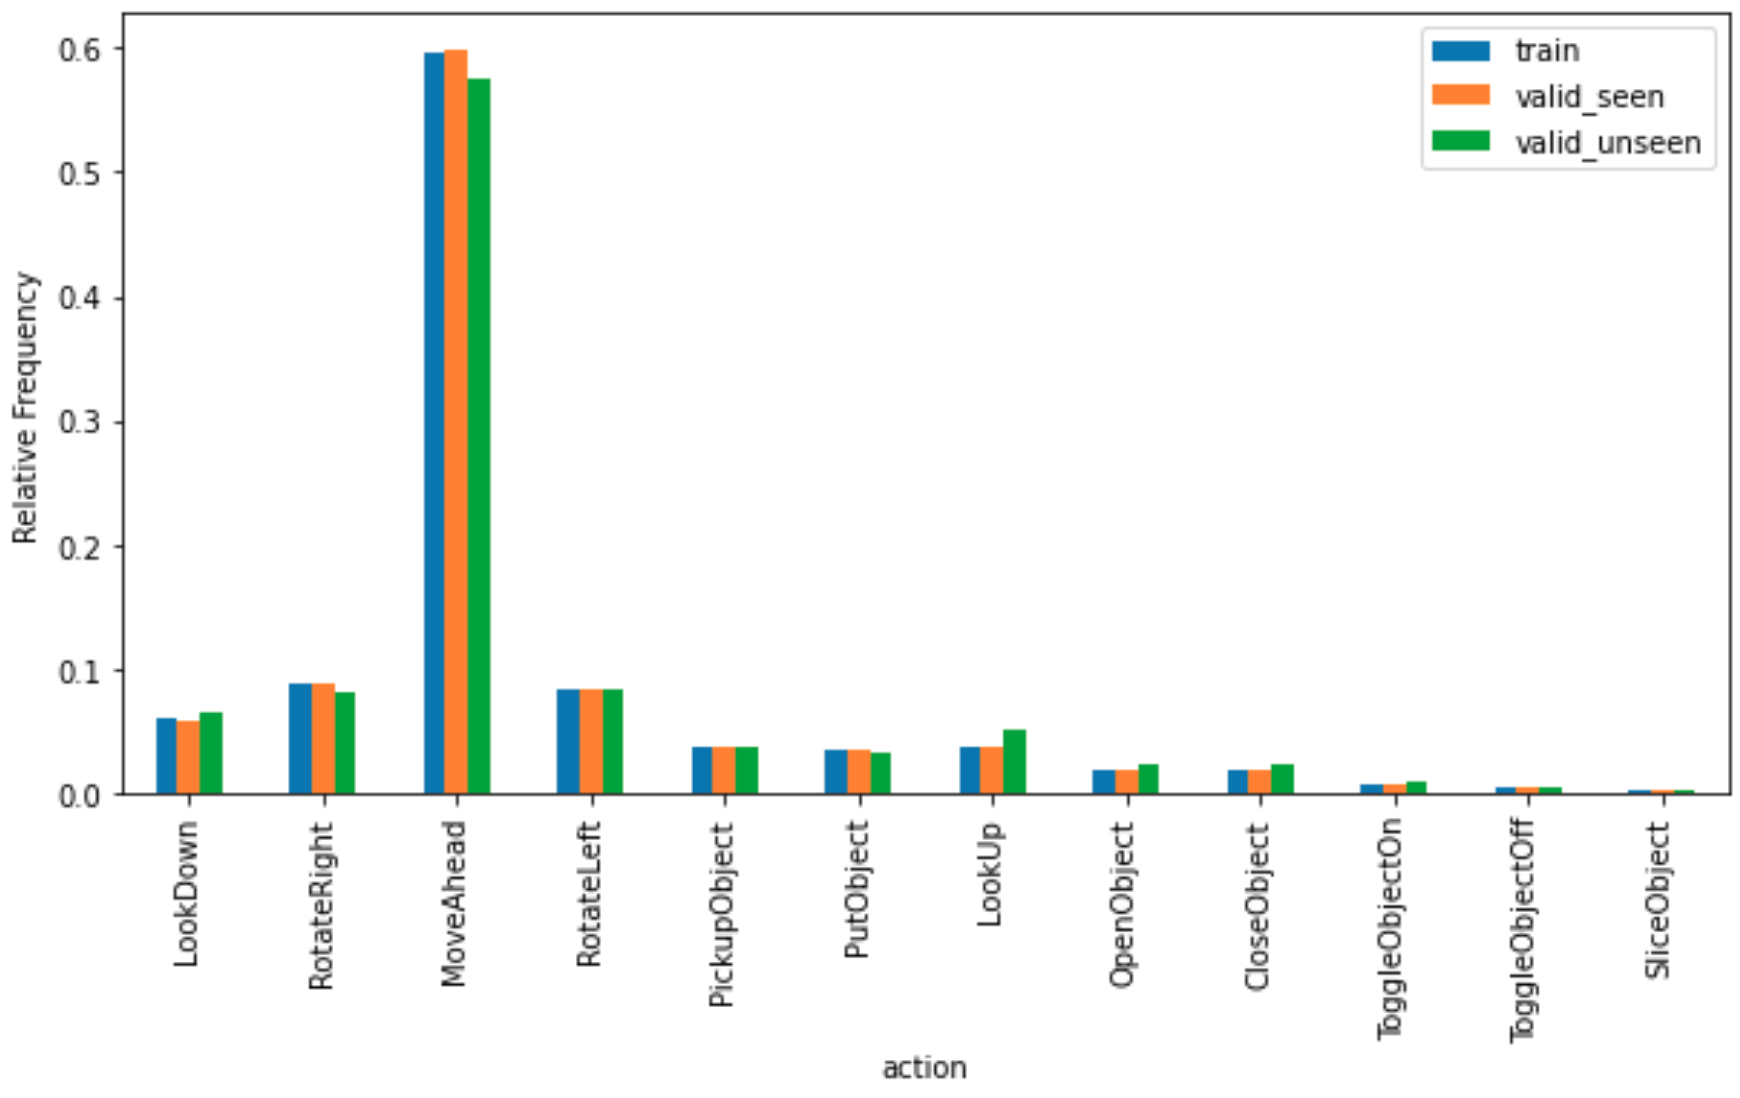
\includegraphics[scale=0.13]{figures/action_freq.png}
\caption{Relative frequency of each action type by split}
\label{fig:action-freq}
\end{figure}

Furthermore, Figure \ref{fig:action-freq} shows the frequency of the 12 different actions (5 navigation actions + 7 interaction actions). Note that all splits have fairly equal frequency for all actions. Also, note that 60\% of actions are ``move ahead'' actions which signifies the importance of a navigation module we may need in our model.

\subsubsection{Textual Analysis}
% important synonyms, and OOV 
For textual analysis, we first identified out of vocabulary (OOV) words in the training and validation set using a vocabulary of 685k words defined by spaCy. We found that less than 0.002\% of all words were OOV in any split, indicating the dataset is already quite clean. Most of the OOV words were just misspelled (eg: "stovve"), indicating that it would be important to preprocess text using a simple spell checker before using it for downstream tasks.

We also found the top few synonyms used to describe objects in the dataset. This was performed by comparing the similarity of word vectors of all objects in the dataset with all common nouns identified in all task descriptions. The complete results are in the Jupyter notebook, but a few results are shown in Table \ref{tab:synonynms}. This reveals that our model will need to be robust enough to recognize synonyms of different words in order to be successful. 

Furthermore, we analyzed how many objects present in the scene are directly referred to in the step-by-step instructions. The results are plotted in a histogram in Figure \ref{fig:object-vs-instruction}, which reveals that much less than 40\% of objects in the scene are actually referred to in the instructions. 

\begin{figure}[H]
\centering
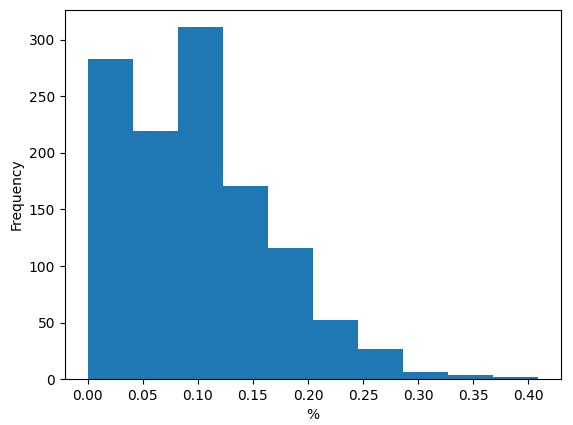
\includegraphics[scale=0.33]{figures/objects_vs_instructions.png}
\caption{Percentage of objects referred to in instructions compared to objects in the scene}
\label{fig:object-vs-instruction}
\end{figure}

\subsubsection{Visual Analysis}
% image sizes, which preprocessing techniques will help, visual quality
Due to compute constraints, most visual analysis was performed qualitatively by inspecting visual quality of different types of images. Figure \ref{fig:sample_ims} shows some sample RGB, depth and instance segmentation images. All images retrieved during simulation are of size 300 x 300.

% We also plan to apply the following three image augmentation methods to increase robustness of our models to unseen data: color jitter (for robustness in unseen lighting conditions), random perspective transformation (for robustness to object being viewed from different angles/perspectives), and random distortion (for general robustness to avoid over-fitting on specific objects seen in training). Note many other common augmentation methods like mirroring and cropping may not be applicable in our setting as they may unrealistically change/hide some objects in the scene.


\begin{table}[H]
\small
\begin{tabular}{@{}ll@{}}
\toprule
Object Name & Synonyms used in task descriptions  \\ \midrule
Coffee Machine & Espresso Machine, Beverage Machine \\
Chair & Couch Chair, Sofa Chair \\
CD   & DVD \\
Side Table & Corner Table \\
Butter Knife & Bread knife \\
Ottomon & Loveseat, Recliner \\
Fridge & Kitchen Fridge, Refrigerator \\
Poster & Wall Photo, Picture \\
Safe & Safety Box \\ 
Soap Bottle & Lotion Bottle
\end{tabular}

\caption{Synonyms (i.e. closest words in embedding space) used in task descriptions of some objects in the dataset}
\label{tab:synonynms}
\end{table}


\begin{figure*}
     \centering
     \begin{subfigure}[b]{0.32\textwidth}
         \centering
         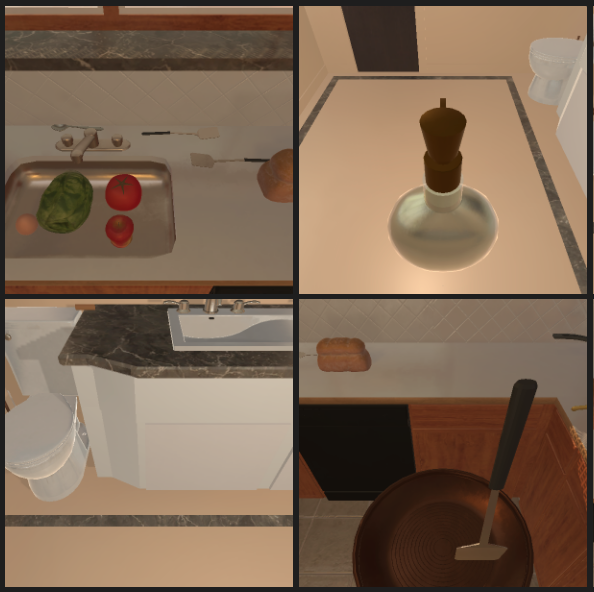
\includegraphics[width=\textwidth]{figures/rgb.png}
         \caption{}
     \end{subfigure}
     \hfill
     \begin{subfigure}[b]{0.32\textwidth}
         \centering
         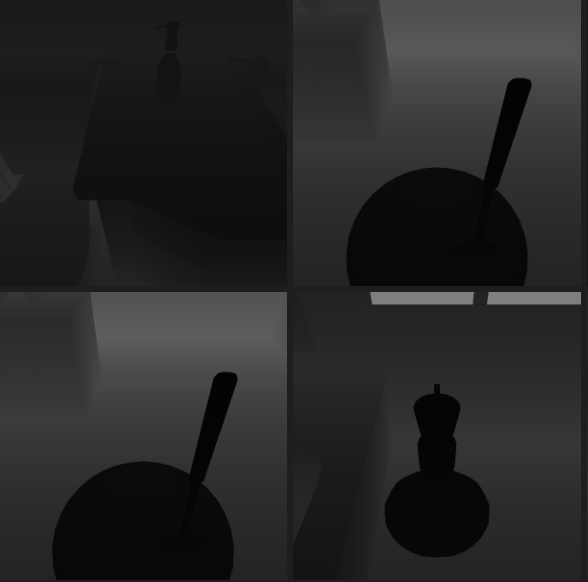
\includegraphics[width=\textwidth]{figures/depth.png}
         \caption{}
     \end{subfigure}
     \hfill
     \begin{subfigure}[b]{0.32\textwidth}
         \centering
         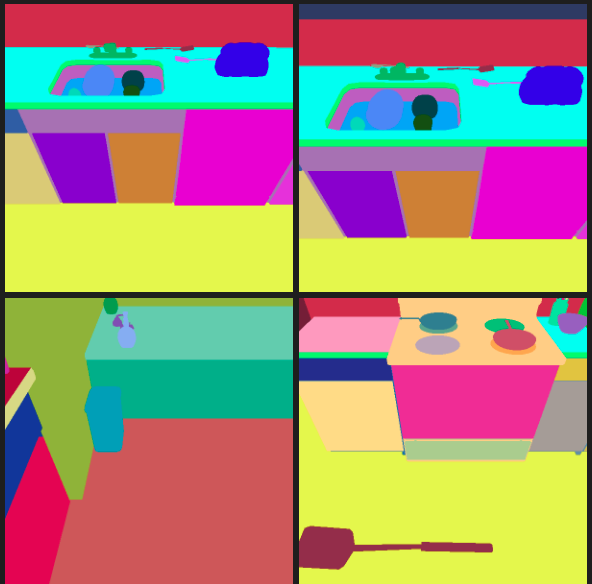
\includegraphics[width=\textwidth]{figures/seg.png}
         \caption{}
     \end{subfigure}
        \caption{Sample RGB, depth, and instance segmentation images retrieved from AI2Thor simulator}
        \label{fig:sample_ims}
\end{figure*}

\subsubsection{Other Qualitative Analysis}
% can a human do that?
In addition to the quantitative analysis, we also analyzed the solvability of the task. Our analysis in Figures \ref{fig:focus} and \ref{fig:dest} (in Appendix) shows that the unseen split of the validation set contains objects from the same classes as the training data, but could contain novel instances of those objects in novel environments. Since classes remain the same during training and testing times, the training data contains full information to solve the task, meaning a sufficiently intelligent agent should be able to solve the task, given training data.

\subsection{Metrics}
There are two primary metrics for evaluation. The first is ``task success'', which is a binary value indicating if the object positions and state changes correspond correctly to the goal-conditions of the task at the end of the action sequence. The second is ``goal-condition success'', which is the fraction of required goal-conditions that were completed at the end of the episode. Note that ``task success'' is true only if ``goal-condition success'' is 100\%. Additionally, there exists a path-weighted version of these two metrics that considers the length of the episode, penalizing longer action sequences. For example, in the path-weighted version, an agent would receive half the score for taking twice as long as an expert to complete the task.
% evaluation methods (Andrew)

\clearpage
\clearpage
\section{Models (2 pages)}

\subsection{Baselines}

% Baselines/Ablations:
    % uni-modal versions of current methods
    % what if we don't use LSTMs?
% Predefined metrics (defined by someone else):
    % All metrics from ALFRED 3.2 section
    % Sub-goal evaluation (as explained in ALFRED)
        % check how this is implemented
        % does this use info from expert trajectories to measure completion of each sub-goal? If yes, which expert trajectory does it use because there are 3?
        % Since most models use some form of LSTM, how can we randomly spawn agents at any place and expect same performance because the LSTM hidden state would not have had a chance to get updated correctly?
% Intrinsic Metrics (defined by us):
    % Navigation: percent of times we reach within distance x of the first object that should be interacted with
        % orientation of agent - is it facing the right object?
    % Interaction Action Prediction: percent of times you predict the right interaction action when you were near the right object
    % Instance Segmentation: given that we are in the right location and we predict the right action, do you get the correct segmentation mask? 
        % group by object class, interaction mask size
    % Length Conditioned Success: the average first n sub-goal achieved without using expert resetting
    % Sub-goal evaluation (as explained in ALFRED) grouped by goal completion index divided by total sub goals
        % plot using x-axis = normalized sub-goal index, y-axis = sub-goal evaluation
        % should also try grouping by task type
        % grouped by action type
    % Note: all metrics can be grouped by task type, seen/unseen, environment type, expert trajectory length (short, medium, long)
    % we can use attention scores to see if the right object is being focused on
        % the exact details of how this will happen are not clear, but can be clarified once the approach is ready
% Empty results table
    % includes all metrics defined above
    % find out which models use depth and image segmentation masks, note this in the results
    % find out if code is available
    % models of interest:
        % moVILAN
        % MOCA
        % ALFRED baseline
        % Modularity improves out of domain generalization
        % Ours
        

\subsubsection{Baselines and Other Methods}
\label{sssec:baselines}
We plan to use the following methods for comparison purposes, which are cited below and explained in Section \ref{sec:rel-work}.

\begin{itemize}
\item \textbf{Seq-2-Seq PM} \cite{shridhar2020alfred} 
\item \textbf{MOCA} \cite{singh2020moca}
\end{itemize}

% \subsubsection{Current Results}
% See Table \ref{tab:results} for baseline and current results on ALFRED.

\subsubsection{Proposed Ablations}
\newcite{shridhar2020alfred} and MOCA \cite{singh2020moca} perform similar input ablation studies for their approaches. They individually remove four inputs from the model: language, vision, the step-by-step instructions, and the goal statement, and evaluate the model's performance in each case. We also plan to conduct a similar ablation study on our model.

In addition, we also plan to perform an ablation study over the training method. While our modeling plans have not been finalized, we currently are interested in exploring an RL-based approach. To empirically verify if RL performs better than IL, we plan to train two variants of our model: one trained using RL, and the other trained using simple IL like other approaches.

\subsubsection{Metrics}
We plan to use the following existing metrics to evaluate our approach.
\begin{enumerate}
    \item \textbf{Task Success}: Task success is simply a binary value indicating whether the final states and positions of objects of interest in the trajectory align with expected states (i.e. if task is completed).
    \item \textbf{Goal-Condition Success}: This is the ratio of goal-conditions completed at the end of the episode to the total number of goal-conditions required for task success.
    \item \textbf{Path Weighted Metrics}: We can also compute the path weighted versions of the above metrics. So, if the model takes twice as many actions has the expert, the original task success and goal-conditioned success scores would decrease by half.
\end{enumerate}

% In addition to computing the above metrics on the entire ALFRED task, we will also compute them at the sub-goal level by moving the agent through the expert trajectory before the sub-goal, and then letting it complete the sub-goal. This was also performed by \newcite{shridhar2020alfred}.

Moreover, to better identify performance bottlenecks in ours and other approaches, we propose the following other metrics:

\begin{enumerate}
    \item \textbf{Navigation Object Success (Nav-Obj)} and \textbf{First Navigation Object Success (First-Nav-Obj)}: Of all the objects the expert interacted with, Navigation Object Success is the proportion of objects that the agent approached at some point in the episode. Here we define ``approached" as coming within a certain distance and facing the correct orientation. We also record whether the agent could approach just the first object that the expert interacted with, denoted by First Object Navigation Success. This metric is important because it more clearly shows whether the agent has at least learned to navigate correctly, which can be measured in a more disentangled manner by only considering navigation to the first object. This is because there will be likely interaction actions before approaching the later objects, making it difficult to reliably attribute credit of future success/failure to navigation alone.

    % Because subsequent actions beyond the first object may involve interaction actions, making it difficult to reliably attribute credit of future success/failure to navigation alone, we also record a True/False of whether the agent approached the first object that the expert interacted with, which we denote First Object Navigation Success. A high value for these metrics indicates that the agent is at least able to successfully navigate to the desired objects, indicating navigation may not necessarily be a performance bottleneck.
    
    \item \textbf{Interaction Success (Int-Succ)}: Interaction Success is the proportion of attempted interactions by the agent that were successful. Note that ``successful" here simply means that the interaction action was executed in the simulator without an API failure. A high value for this metric indicates that the agent is able to at least successfully predict an appropriate action and interaction mask to interact with objects, even if they may not necessarily be objects that are relevant to the goal.
    
    \item \textbf{Bad Mask Failure Rate (Bad-Mask)}: Bad Mask Failure Rate is the proportion of interaction failures that were due to a bad interaction mask. A high value indicates that the primary obstacle to an agent successfully interacting with objects is the interaction mask, while a low value indicates that most of the interaction failures are due to a different reason, such as incorrect action prediction (see item 5: Interaction Action Prediction Success).

    \item \textbf{Unnecessary Interaction Ratio (Unnec-Int)}: Unnecessary Interaction Ratio is defined as the number of  objects the agent interacted with that the expert did not, divided by the number of objects the expert interacted with. A high value will reveal that the agent is interacting with proportionally many objects not relevant to the task, while a low value indicates that the agent is focusing on the objects that are relevant to completing the task.
    
    \item \textbf{Interaction Action Prediction Success (Int-Act-Pred)}: Interaction Action Prediction Success is the fraction of times the model predicts the right interaction action given that it has identified the instance segmentation mask of the correct object. A high value for this metric indicates that once the agent can produce a correct mask, the task of predicting which action to execute is not a bottleneck. A low value suggests that even when the agent is able to produce a correct mask, predicting which action to take is still a significant obstacle to successful interaction.
\end{enumerate}

Note that a recurring theme in most proposed metrics is to measure performance over each aspect needed to solve the task in as much isolation as possible. % For example, we try to measure navigation and interaction performance separately by using NP, IMPP, and IAPP as proposed above.

In addition to the above base metrics, we also plan to group all metric calculations by task type to understand models at a more fine-grained level.

\subsubsection{Results table}
As mentioned in \ref{sssec:baselines}, we compare our approach to two other approaches. We report our overall results in Table \ref{tab:results}. Additionally, we report results for our proposed intrinsic metrics on the validation set and compare to the baseline model in Table \ref{tab:intrinsic}, and analyze them in Section \ref{ssec:insights}.

\subsection{Qualitative Analysis}
We also ran the baseline and MOCA policy on a few examples to qualitatively analyze the agent's performance. The screen recordings of these examples are uploaded on Google drive, and linked below.

In example 1, titled \href{https://drive.google.com/file/d/1xXIIFGBwzP2QGCXlV4v_YlFTHf9C8228/view?usp=sharing}{Base-Ex1}, the agent has to take a spray bottle from the basin counter and place it on the toilet. Instead, the agent picks up a cloth (placed near the spray bottle) from the basin counter and just moves on the other end of the counter. Note that even though the agent moved correctly to the spray bottle and made only a small mistake (i.e. picked up cloth instead of spray bottle), it could not recover from the mistake, and ended up doing something very different at the end. This highlights a common problem with vanilla imitation learning that the agent cannot recover from small mistakes because that are out of training distribution.

% In the second task, titled \href{https://drive.google.com/file/d/1EBtl4o32FOcBZlhw9CHX83WBGpgXCzCj/view?usp=sharing}{Base-Ex2}, the agent is supposed to pick up two spatulas (one after another) and place them in a drawer. Instead, the agent picks up a loaf (not placed near spatula) of bread and completes a U-turn, which simply highlights how little the agent understands the task.

In the next example, titled \href{https://drive.google.com/file/d/1A790sCe33eKV-MivCO2t5O2DD8Atlh2C/view?usp=sharing}{Base-Ex3}, the agent is supposed to microwave a potato and put it in the fridge. Instead, the agent starts a length trajectory without every picking up the potato: It opens, operates, and closes the microwave repeatedly (sometimes placing nothing inside of it) and then repeatedly opens and closes the fridge (placing nothing inside of it). This example (and many others we have seen) highlight the primitiveness of the agent, and show that the agent is not really learning anything useful, but just operating on statistical co-occurrences: for example, whenever it sees a fridge/microwave, it just repeats a particular action sequence (i.e. open, put object inside, close for fridge or open, put object inside, close, turn on, pick object up, turn off).

The MOCA policy does perform relatively better than the baseline, but the same problems mentioned are noticed. In example \href{https://drive.google.com/file/d/16_FJ3689Mv5dxvu9pU1HZ96QvNm7fCc2/view?usp=sharing}{Moca-Ex4} the agent is asked to slice an apple in the pan with a knife; instead it picks up a fork and travels back and forth in the kitchen. As with baseline, the agent makes a mistake by picking up the fork but is not able to recover from the mistake made early on.

In the next example, \href{https://drive.google.com/file/d/1F400UjTNvMC2pw7HWOOEJ3va-XKUu0nE/view?usp=sharing}{Moca-Ex5} the agent is asked to take a mug, microwave it, and place it on the table across the room again. Unfortunately, the agent simply walks in loops inside the kitchen without even trying to pick up the mug. Similar to the baseline policy, this example reveals that the policy is not really learning anything intuitive, and is not able to attend over the correct objects in long, complex trajectories.

\subsection{Inferences, Interpretations, and Insights}
\label{ssec:insights}
In this section, we analyze the implications of both our quantitative and qualitative results.

\textbf{Intrinsic Metrics (Table \ref{tab:intrinsic})} 
\begin{enumerate}
    \item Navigation remains a challenge on unseen data. On the unseen split, even MOCA is unable to navigate to the first relevant object one-third of the times, and only navigates to just over half of the relevant objects throughout the episode. However, the fact that MOCA performs significantly better than the baseline model on the unseen split suggests that the language-guided dynamic filters and obstruction detection that MOCA adds could be beneficial to generalizing navigation to new environments.
    \item Failed interactions are a bottleneck to overall performance on unseen data. We see that even MOCA has just a 24.5\% interacton success rate on the unseen split, while the baseline has a lower 14.8\% success rate. In the case of MOCA, most of these failures (73.7\%) are due to incorrect masks, while just under half are for the baseline. Given that one of MOCA's key contributions is a novel module for object-centric mask prediction, this is somewhat surprising. This could however be explained if the baseline model first encounters other failure modes that MOCA is able to overcome, so the baseline is not able to reach the point where the interaction mask is the bottleneck. Looking further into the data, we find that MOCA attempted nearly $2.5\times$ more interactions than the baseline did, suggesting that perhaps other bottlenecks such as navigation are limiting the baseline's potential for interacting with objects (see item 1).
    \item These models do not focus well on the objects relevant to the goal, interacting with roughly the same number of irrelevant objects as there are relevant objects in the trajectory (shown by the Unnecessary Interaction Ratio of roughly 1 for both models). This suggests that these models are not successfully integrating the language directives with their perceptual inputs to select the objects specified by the directives.
    \item Action prediction remains a significant bottleneck to successful interaction, especially on unseen data. Even after producing a correct interaction mask, MOCA still only predicts the correct interaction action 14\% of the time, and the baseline only 0.8\% of the time, on the unseen split. This suggests that while mask prediction is a significant challenge, an equally (if not more) important task is predicting the correct action to take to interact with the object.
\end{enumerate}

\textbf{Task-Level Metrics by Task Type}
We group the two task-level metrics, Task Success and Goal-Condition Success, by the 7 task types in ALFRED and plot the results in Figures \ref{fig:ts-by-type} and \ref{fig:gcs-by-type}. While the baseline model struggles with all task types, MOCA demonstrates a substantial improvement on all tasks in the seen split except on the \textbf{Stack \& Place} task. This could be due to the fact that \textbf{Stack \& Place} is the only task with a movable receptacle, presenting a unique challenge that is not found in other tasks. 

The task that both models perform best on is the \textbf{Clean \& Place} task. In the unseen split, MOCA interestingly performs much better on this task than on any other task type. Further exploration of the unique attributes of this task may be needed to determine why MOCA's success rate is so much higher on the unseen split than other tasks. Perhaps it is because this task has less change from seen to unseen than the other tasks, or perhaps it is simply due to variability in the evaluation: the raw number of successes for MOCA on this task in the unseen split was just 18, and was 1-5 for the other tasks.

The key insight from these plots is that for many task types, a substantial improvement in seen performance does not necessarily imply the same improvement in unseen performance. Learning how to successfully generalize to new environments and objects is a distinctive challenge and must be addressed explicitly when designing an approach.

\textbf{We also did a similar task level analysis on metrics we designed ourselves (not discussed due to space constraints), and the results of the same are provided in a \href{https://github.com/ankit61/group-tars-alfred/blob/main/Reports/4-Analysis-of-Baselines/results_analysis.ipynb}{Jupyter notebook} added in the submission folder.}

\begin{figure}[H]
\centering
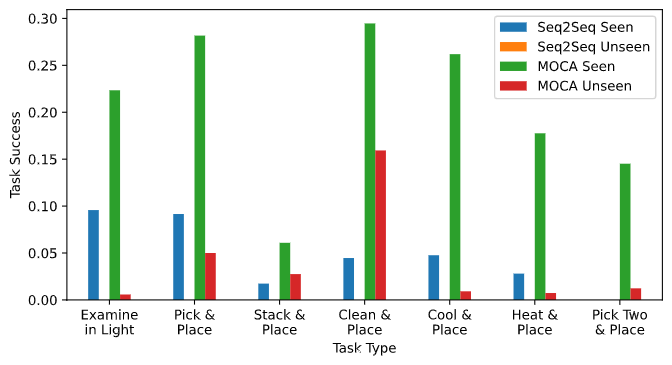
\includegraphics[scale=0.33]{figures/ts_by_type.png}
\caption{Task Success by Task Type}
\label{fig:ts-by-type}
\end{figure}

\begin{figure}[H]
\centering
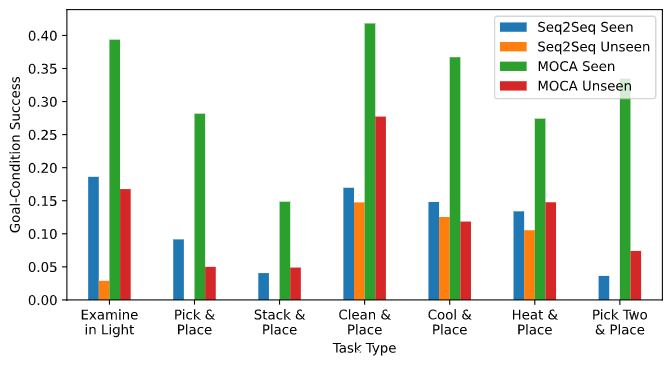
\includegraphics[scale=0.33]{figures/gcs_by_type.png}
\caption{Goal-Condition Success by Task Type}
\label{fig:gcs-by-type}
\end{figure}


\textbf{Need for RL.} The most important lesson we learned from our analysis was just how important RL could be for this task. Below we highlight specific reasons we think that RL is crucial for solving a multimodal navigation and interaction task like ALFRED:

\begin{enumerate}
    \item Our qualitative analysis highlights cases where the agent makes one mistake and cannot recover from it because it has deviated too much from the expert trajectory and does not have enough information to get back on the right course. This is a common problem that imitation learning agents face \cite{ross2011reduction}, and something RL agents typically won't suffer from because they are trying to maximize a reward instead of rote learn a trajectory.
    \item Since supervision in RL comes from a self designed reward function, we can force the agent to learn much more task specific knowledge compared to the vanilla imitation learning. For example, Table \ref{tab:intrinsic} shows that in most cases agents trained with both MOCA and baseline agents interact with more unnecessary objects than the total objects needed to complete the task (because Unnec-Int is often greater than 1). This is of course an undesirable behavior, but one that cannot be controlled by imitation learning directly. In case of RL, we could simply give a negative reward to the agent for all unnecessary interactions, making the agent explicitly learn that such behavior is undesired.
\end{enumerate}


\begin{table*}[]
\centering
\resizebox{\textwidth}{!}
{\begin{tabular}{@{}lllllllll@{}}
\toprule
                         & \multicolumn{4}{c}{\textbf{Validation}}                                                                             & \multicolumn{4}{c}{\textbf{Test}}                                                                                   \\
                         & \multicolumn{2}{c}{\textit{Seen}}                        & \multicolumn{2}{c}{\textit{Unseen}}                      & \multicolumn{2}{c}{\textit{Seen}}                        & \multicolumn{2}{c}{\textit{Unseen}}                      \\
Model                    & \multicolumn{1}{c}{Task} & \multicolumn{1}{c}{Goal-Cond} & \multicolumn{1}{c}{Task} & \multicolumn{1}{c}{Goal-Cond} & \multicolumn{1}{c}{Task} & \multicolumn{1}{c}{Goal-Cond} & \multicolumn{1}{c}{Task} & \multicolumn{1}{c}{Goal-Cond} \\ \midrule
Seq2Seq + PM Both \cite{shridhar2020alfred}                & 3.70 (2.10)              & 10.00 (7.00)                  & 0.00 (0.00)              & 6.90 (5.10)                   & 3.98 (2.02)              & 9.42 (6.27)                   & 0.39 (0.80)              & 7.03 (4.26)                   \\
Modular \cite{corona2020modularity}          & \multicolumn{1}{c}{-}    & \multicolumn{1}{c}{-}         & \multicolumn{1}{c}{-}    & \multicolumn{1}{c}{-}         & \multicolumn{1}{c}{-}    & 8.80 (6.30)                   & \multicolumn{1}{c}{-}    & 7.20 (5.70)                   \\
MOCA \cite{singh2020moca}                     & 19.15 (13.60)            & 28.50 (22.30)                 & 3.78 (2.00)              & 13.40 (8.30)                  & 22.05 (15.10)            & 28.29 (22.05)                 & 5.30 (2.72)              & 14.28 (9.99)                  \\
\textbf{Ours}            &                          &                               &                          &                               &                          &                               &                          &                               \\ \midrule
Human                    & \multicolumn{1}{c}{-}    & \multicolumn{1}{c}{-}         & \multicolumn{1}{c}{-}    & \multicolumn{1}{c}{-}         & \multicolumn{1}{c}{-}    & \multicolumn{1}{c}{-}         & 91.00 (85.80)            & 94.50 (87.60)                 \\ \midrule
\textbf{Ablations} &                          &                               &                          &                               &                          &                               &                          &                               \\
No Language              &                          &                               &                          &                               &                          &                               &                          &                               \\
No Vision                &                          &                               &                          &                               &                          &                               &                          &                               \\
Goal-Only                &                          &                               &                          &                               &                          &                               &                          &                               \\
Instructions-Only        &                          &                               &                          &                               &                          &                               &                          &                               \\
Trained using IL only       &                          &                               &                          &                               &                          &                               &                          &                               \\\bottomrule
\end{tabular}}
\caption{\textbf{Task and Goal-Condition Success Rate.} Corresponding path-weighted metrics are given in parentheses.}
\label{tab:results}
\end{table*}

\begin{table*}[]
\centering
\resizebox{\textwidth}{!}{%
\begin{tabular}{@{}lllllllllllll@{}}
\toprule
                      & \multicolumn{6}{c}{\textit{Seen}}                                                                                                                             & \multicolumn{6}{c}{\textit{Unseen}}                                                                                                      \\ \midrule
Model                 & Nav-Obj                   & First-Nav-Obj               & Int-Succ                  & Bad-Mask             & Unnec-Int & \multicolumn{1}{l|}{Int-Act-Pred} & Nav-Obj                   & First-Nav-Obj               & Int-Succ                & Bad-Mask             & Unnec-Int & Int-Act-Pred \\ \midrule
Seq2Seq + PM Both     & \multicolumn{1}{r}{0.680} & \multicolumn{1}{r}{0.735} & \multicolumn{1}{r}{0.494} & \multicolumn{1}{r}{0.250} & 1.298     & \multicolumn{1}{l|}{0.131}        & \multicolumn{1}{r}{0.283} & \multicolumn{1}{r}{0.322} & \multicolumn{1}{r}{0.148} & \multicolumn{1}{r}{0.437} & 0.809     & 0.008        \\
MOCA                  & \multicolumn{1}{r}{0.778} & \multicolumn{1}{r}{0.838} & \multicolumn{1}{r}{0.470} & \multicolumn{1}{r}{0.617} & 1.103     & \multicolumn{1}{l|}{0.279}        & \multicolumn{1}{r}{0.586} & \multicolumn{1}{r}{0.669} & \multicolumn{1}{r}{0.245} & \multicolumn{1}{r}{0.737} & 1.375     & 0.140        \\
\textbf{Ours}         &                           &                           &                           &                           &           & \multicolumn{1}{l|}{}             &                           &                           &                           &                           &           &              \\ \midrule
\textbf{Ablations}    &                           &                           &                           &                           &           & \multicolumn{1}{l|}{}             &                           &                           &                           &                           &           &              \\
No Language           &                           &                           &                           &                           &           & \multicolumn{1}{l|}{}             &                           &                           &                           &                           &           &              \\
No Vision             &                           &                           &                           &                           &           & \multicolumn{1}{l|}{}             &                           &                           &                           &                           &           &              \\
Goal-Only             &                           &                           &                           &                           &           & \multicolumn{1}{l|}{}             &                           &                           &                           &                           &           &              \\
Instructions-Only     &                           &                           &                           &                           &           & \multicolumn{1}{l|}{}             &                           &                           &                           &                           &           &              \\
Trained using IL only &                           &                           &                           &                           &           & \multicolumn{1}{l|}{}             &                           &                           &                           &                           &           &              \\ \bottomrule
\end{tabular}%
}
\caption{Intrinsic Metrics - Validation.}
\label{tab:intrinsic}
\end{table*}


\subsection{Other noteworthy details}
We want to highlight that there were certain baseline models and metrics that we had planned to do in this submission, but could not due to various reasons such as implementation feasibility, compute limits, etc. We explain specific reasons why those baselines and metrics could not be computed in the appendix Section \ref{app:missed}.

Moreover, we want to highlight that we built a full end to end pipeline to perform our analysis, which contains clean, refactored and generalizable  versions of the baseline Seq2Seq model \cite{shridhar2020alfred} and MOCA \cite{singh2020moca}. The current implementation of the baseline Seq2Seq model \cite{shridhar2020alfred} is quite complicated and very tightly intertwined with specific other code in their library. These factors implicitly force all other ALFRED models to be coded up in a very specific manner, so they can use the evaluation scripts provided by the original ALFRED authors. For example, the MOCA model is also implemented using same ALFRED code because of tight coupling within different parts in that code base (such as dependence of models on specific styles of data preprocessing).  We feel this is suboptimal because such coding styles hinder generality. For example, it is not (easily) possible in the original code base to train the same proposed baseline model as a policy network using reinforcement learning. Therefore, we designed our pipeline that can take any model and potentially train it using both reinforcement learning and/or imitation learning. We want to highlight that the actual training code has not be written because that was not the goal of this milestone, but the interface is generic enough to support it. We highlight important features of our pipeline in appendix Section \ref{app:code}.

\subsection{Proposed Approach}

\subsubsection{Motivation}
\label{ssec:motiv}

We noticed that in all proposed ALFRED models, there is a significant reliance on phenomena that the authors expect would automatically emerge without explicit enforcement, and little focus on grounding of different modalities. In the following, we identify concrete instances of such over-reliance on emergent phenomena and little focus on grounding.

\begin{itemize}
    \item \textbf{Too much reliance on LSTM hidden state.} In the original baseline model \cite{shridhar2020alfred} (see Figure \ref{fig:alfred_model}), the LSTM's (shown in green in the figure) hidden state's role is to keep track of current context (as it is used to attend over instructions). However, to perform well in the task, a lot of information needs to be included in the ``context''. For example, ``context'' needs to include some action history, interaction history, instruction understanding, goal understanding, and image understanding with respect to the goal and instruction, among other things. It seems quite unlikely that such a rich representation will automatically emerge in the hidden state, especially without any enforcement. Note that such an argument can be made even for the LSTMs used in the MOCA \cite{singh2020moca} architecture.
    \item \textbf{Little benefit from previous action.} Both MOCA \cite{singh2020moca} and the baseline model \cite{shridhar2020alfred} (see Figures \ref{fig:moca_model} \& \ref{fig:alfred_model}) use the previous action in their model as input to better provide context to the model.  Based on our data analysis, using only the most recent action seems to be ineffective since 60\% of actions are just "MoveAhead"; in other words, 60\% of the time the model cannot extract very meaningful information from the most recent action alone. Furthermore, for interaction actions, keeping track of the action alone does not provide any information about the object that the agent interacted with. Due to these reasons, the burden of the LSTM to maintain an informative context increases even further because all extra information is expected to be stored in its hidden state.
    \item \textbf{Language not grounded in vision.} Both the baseline model and MOCA do not ground language in vision (MOCA grounds vision in language using dynamic filters, but not vice versa). It seems that grounding language in vision (in addition to grounding language in the current context) is essential because visual input directly can tell the model what is visible in the scene, and what to focus on in language accordingly.
\end{itemize}

As we will describe, we attempt to solve all above issues in our proposed model.

\subsubsection{Notation}
\label{sssec:notation}
Before we discuss our model, we introduce some notation that would make describing the model easier:

\begin{itemize}
    \item $G$ denotes the natural language description of the high level goal of the task. So, $G = [g_1, \dots, g_{|G|}]$ where $g_i$ denotes the $i^{th}$ word.
    \item $L$ denotes the list of step-by-step natural language instructions. So, $L = [L_1, \dots, L_{|L|}]$ such that each $L_i$ is the $i^{th}$ instruction, and $L_i = [L_{i1}, \dots, L_{in}]$ where $L_{ij}$ denotes the $j^{th}$ word of the $i^{th}$ instruction.
    \item $I_t$ is the RGB image from the simulator at the $t^{th}$ time step.
    \item $(a_t, O_t)$ is a tuple such that $a_t$ denotes the action taken at time step $t$, and $O_t$ denotes the class of the object upon which the action was applied in case the action was an interaction action.
    \item $M_t$ is the interaction mask corresponding to particular instance of object from class $O_t$.
    \item $O_{I_t}$ denotes the list of object names visible in image $I_t$. So, $O_{I_t} = \{O_{I_t}^1, \dots, O_{I_t}^k\}$ where $O_{I_t}^i$ is the $i^{th}$ object in the scene (with no particular order). As will be described later, $O_{I_t}$ is retrieved by running instance segmentation \cite{he2017mask} on $I_t$ and getting object class names.
\end{itemize}

\subsubsection{Proposed Idea}
\label{sssec:proposed}
Using the described notation, Figure \ref{fig:model} shows the complete architecture, and we explain each element and modelling choice below.

\begin{itemize}
    \item \textbf{Disentangling Explicit \& Implicit Context.} An important novel contribution of our method is to significantly lighten the load of each LSTM. As described in Section \ref{ssec:motiv}, current architectures expect too much from their LSTMs. To this end, we provide some easily deducible history directly to our model, so the LSTM can only focus on learning a more latent and abstract form of context. This lets us essentially disentangle the explicit and implicit forms of context, which should make learning much simpler.

    Specifically, we intend to pass the last $k$ actions and the last $k'$ objects the agent interacted with as input.  As shown in the context module of Figure \ref{fig:model}, we will use these two inputs to construct a representation of ``explicit context''. We can combine this ``explicit context'' with the hidden states of our two LSTMs (which together form a representation of ``implicit context'') that will be explained below to form an overall context vector. We can then use this overall context vector to perform attention over natural language instructions and goal as shown in the figure.  The intuition behind passing the last few actions and interaction objects is that any agent would need to keep track of its last few actions and interactions to have a good understanding of what its doing, so it makes more sense to just directly provide this history.

    \item \textbf{Grounding Language in Vision.} We propose to use a novel multimodal method to ground language in vision. Our insight is that it would be much harder for the model to align a raw visual representation (obtained from running a simple CNN on the input image) with a language representation because vision and language features are inherently different. If we can represent the image well using language, it would be much easier to align it with the instructions because both would be sequences of linguistic features. Our solution is to run an instance segmentation model on the input image $I_t$ and identify all objects in the image (represented by $O_{I_t}^1, \dots, O_{I_t}^k$ in the vision module of Figure \ref{fig:model}). Since these objects are just words, we can embed them using pre-trained word embeddings and then run these embeddings through a transformer (without positional encodings because there is no inherent order) to get an overall representation (called ``object embedding'' in Figure \ref{fig:model}). As shown in the figure, we use these embeddings and raw vision features to get ``overall vision features'', which are later used to attend over the natural language instructions as shown in the Action Module. We feel that language grounding would be much easier if we directly identify all objects in the image by their names because a) we are aligning language features with language features instead of vision features with language features, b) we are directly providing all objects in the scene as input, thereby significantly reducing the load of the CNN that outputs the ``raw vision features'' in Figure \ref{fig:model}. While we thought of this idea independently, we would like to point out that the idea of using object labels has been used in a previous ALFRED model \cite{Storks2021AreWT}, but in a different way. While \newcite{Storks2021AreWT} used this idea in a small module which was used to input additional features to the original baseline model \cite{shridhar2020alfred}, our idea has no dependence on the baseline model.

    \item \textbf{Two LSTMs.} Instead of using only one LSTM as in the baseline model \cite{shridhar2020alfred}, we propose to use two different LSTMs: one to keep track of instructions, and another to keep track of the high level goal description as shown in the Action Module of Figure \ref{fig:model}. Having two LSTMs again significantly reduces the responsibility of each because a clear disentanglement can be achieved between low level instruction following and high level goal completion. As shown in the figure, the low level ``instruction LSTM'' is responsible for action and interaction object prediction based on overall context, vision features, and attended low level natural language instructions. The ``goal LSTM'' is then updated using the predicted action and object, and the natural language goal description is attended based on the overall context. Note that MOCA also uses two LSTMs as shown in Figure \ref{fig:moca_model}, but the LSTMs do not interact with each other, and they serve a very different intuitive purpose (keep track of perception and policy) than the two LSTMs in our model (keep track of overall goal and low level instructions).

    \item \textbf{Interaction Mask Prediction.} We follow MOCA's \cite{singh2020moca} approach of disentangling object class prediction and instance mask prediction. This makes the action predictor's job significantly easier because it only needs to identify the class of the object it needs to interact with (which often would be mentioned directly in natural language instructions) instead of identifying the object class, identifying the object in the current image, and then predicting a segmentation mask around the object. We plan to use MOCA's exact method of associating the actual object instance from the predicted object class using confidence and association-based measures.

    \item \textbf{Mini Transformer + Readout} At various places in our model, we use a mini transformer to obtain one cumulative representation out of a given set of representations. We use the word ``mini'' to denote that we just intend to use 2-3 layers of the transformer instead of all 12.  As shown in Figure \ref{fig:model}, we use an additional input (denoted by $\mathcal{R}_1, \mathcal{R}_2, \mathcal{R}_3$) in all mini transformers. $\mathcal{R}_i$ is simply a learned vector added to each transformer, and serves the same role as a classification token does in BERT \cite{devlin2018bert}. The additional token is just used to \emph{readout} a vector (denoted by $\hat{\mathcal{R}_i}$) from the output of the transformer, which can then be used for downstream processing. This mini transformer + readout block is used whenever we want the input sequence to be processed with respect to other elements of the sequence. For example, it is important to process past actions with respect to each other so that the model knows exactly what the agent was trying to do in the past.

\end{itemize}

\begin{figure*}
    \centering
    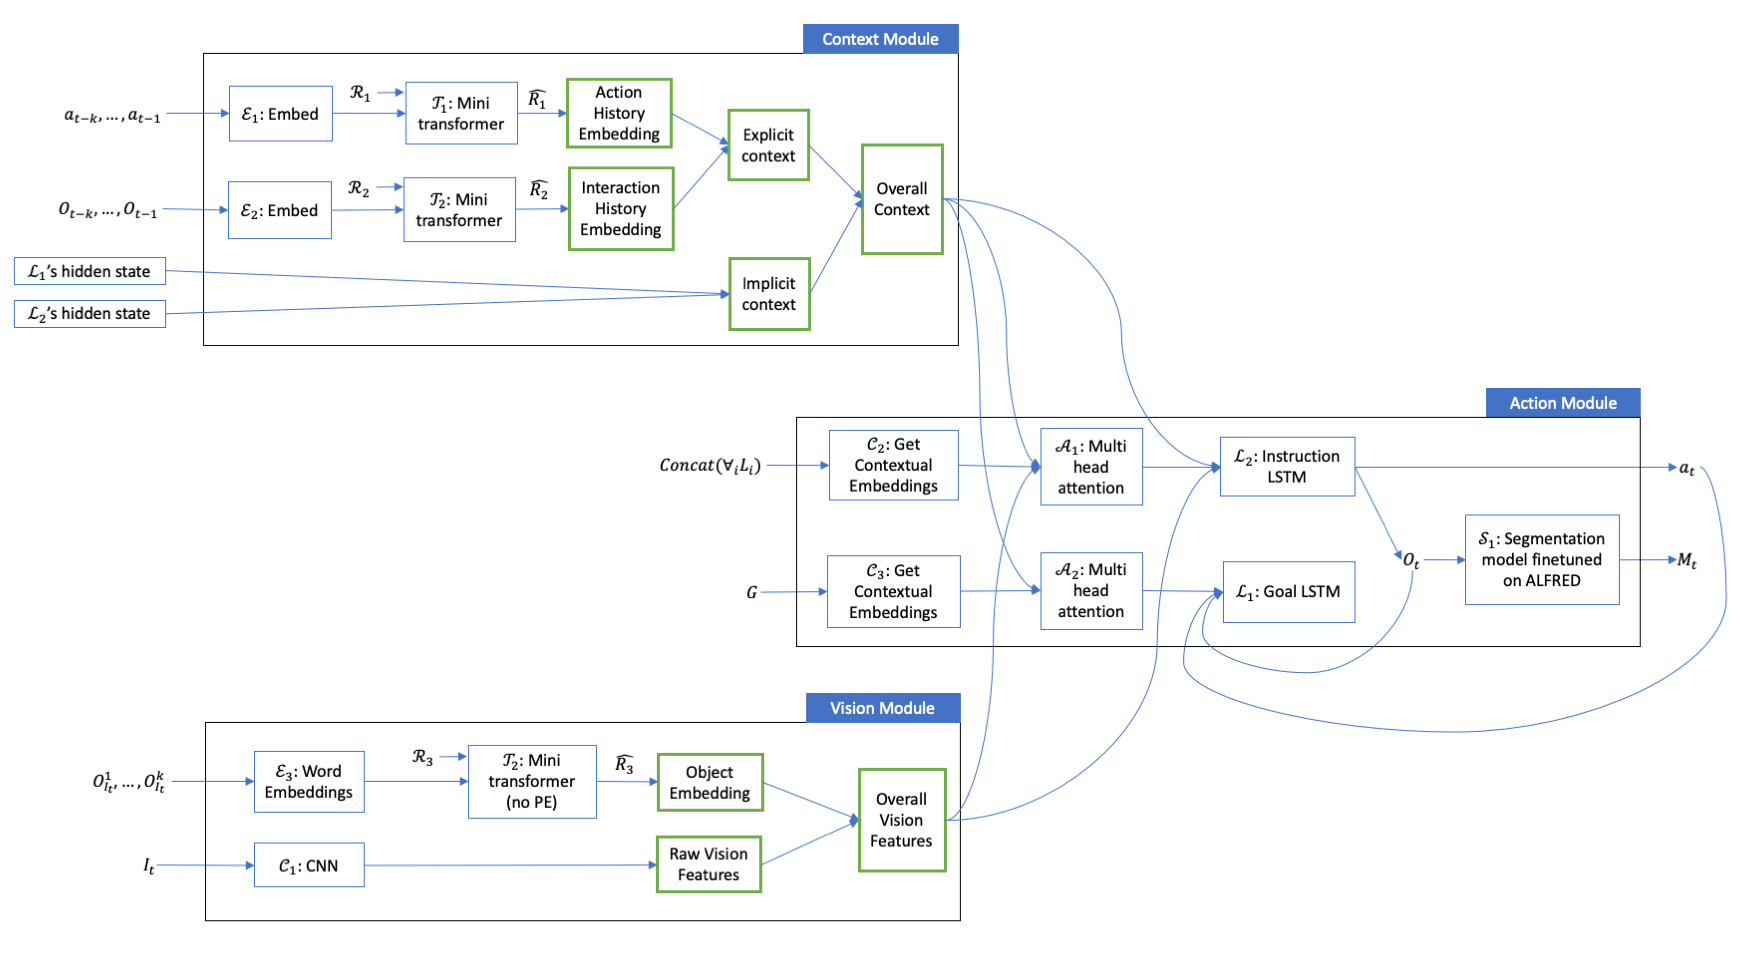
\includegraphics[scale=0.4]{figures/our_model.png}
    \caption{Our proposed model consists of three novel modules as shown which are intended to provide better overall structure, stronger inductive biases, and more prior information to make it easier for each part of the model to learn. The notation used here is described in Section \ref{sssec:notation}, and the model is explained in detail in \ref{sssec:proposed}.}
    \label{fig:model}
\end{figure*}


\clearpage

\section{Results (1 page)}
The columns above are just examples that should be expanded to include all metrics and baselines.

\clearpage
\section{Analysis (2 pages)}
This section should include at least two to three plots
\subsection{Ablations and Their Implications}

\subsection{Qualitative Analysis and Examples}
This section should likely contain a table of examples demonstrating how the current approach succeeds/fails.

% Please use 
\bibliographystyle{acl_natbib}
\bibliography{references}

%\appendix
\clearpage
\section{Appendix}

\begin{figure*}
    \centering
    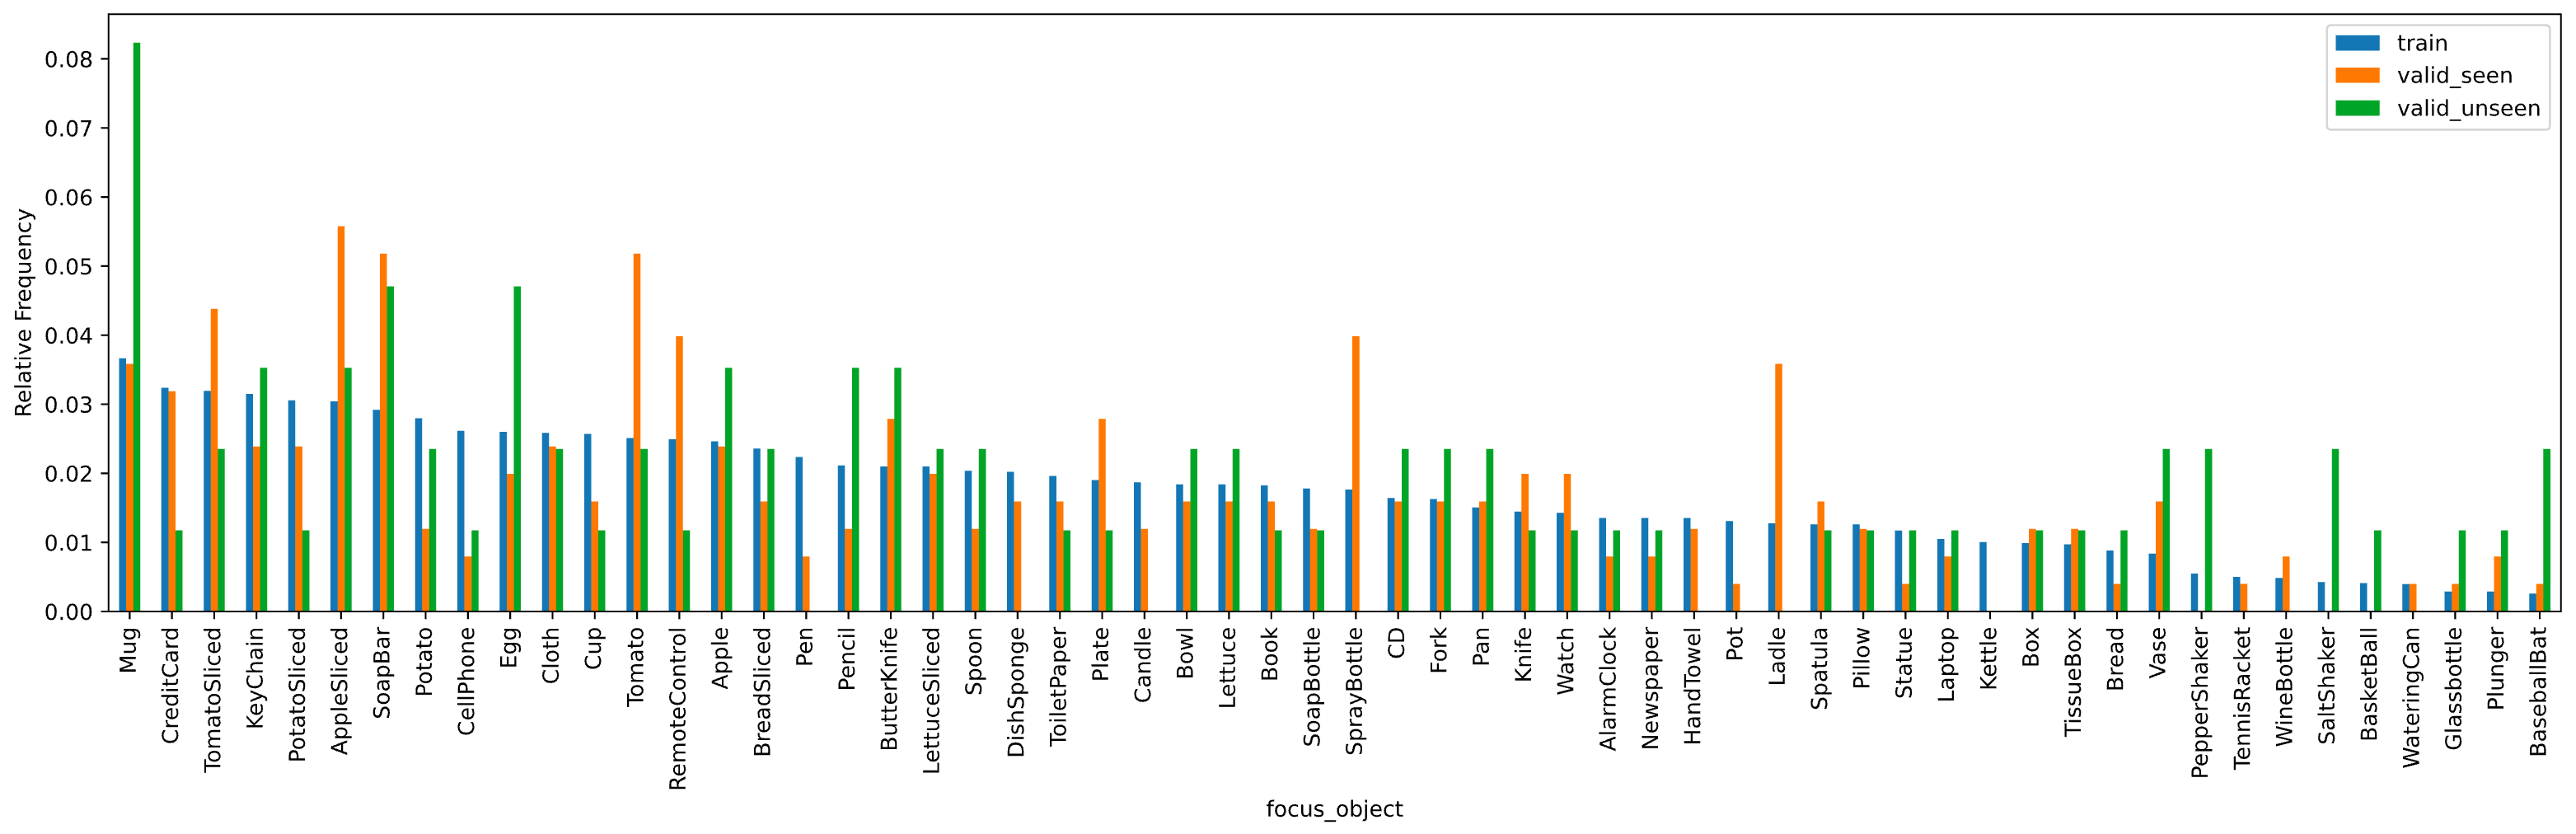
\includegraphics[scale=0.3]{figures/focus_obj_freqs.png}
    \caption{Relative frequency of focus objects used in different splits}
    \label{fig:focus}
\end{figure*}

\begin{figure*}
    \centering
    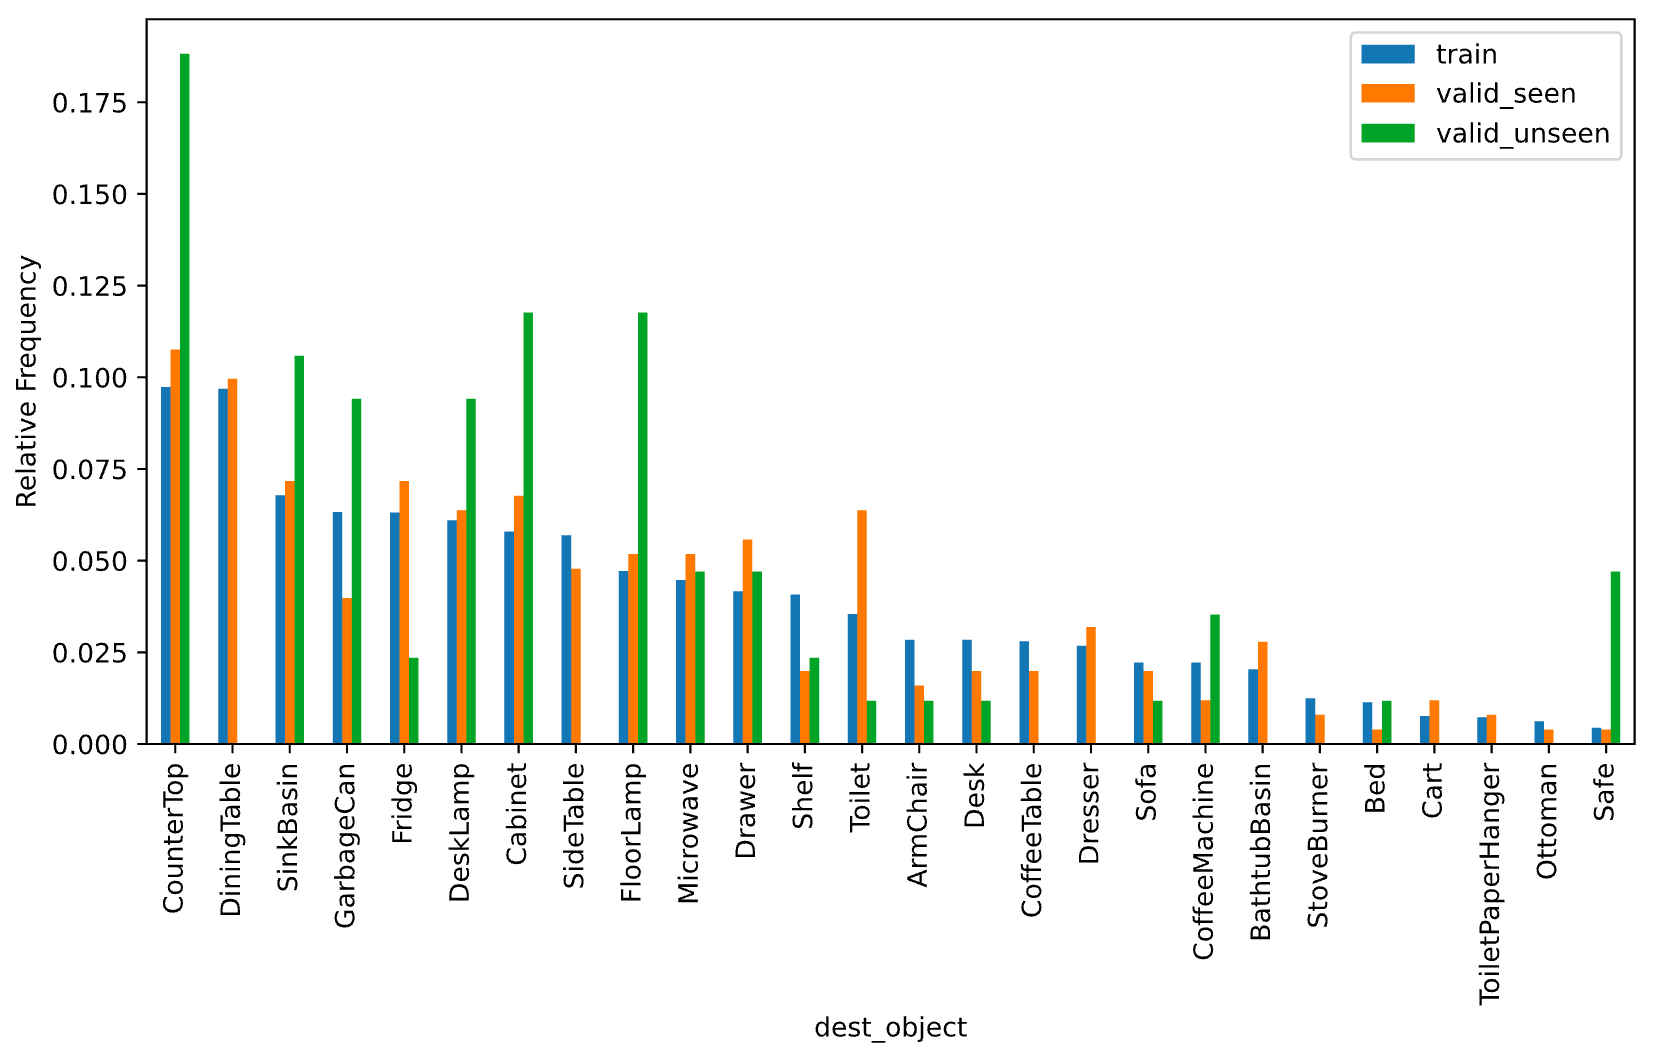
\includegraphics[scale=0.5]{figures/dest_obj_freqs.png}
    \caption{Relative frequency of destination objects used in different splits}
    \label{fig:dest}
\end{figure*}


\subsection{Data Analysis Plots}

Description of fields in Table \ref{fig:action-freq}:
\begin{enumerate}
    \item Steps per directive: number of steps in each language directive
    \item Tokens per step: number of words in each directive step
    \item Task description tokens: number of words in directive task description
    \item Images: number of images per demonstration
    \item Actions: number of actions per demonstration
    \item Images per action: number of images divided by number of actions per demonstration
    \item Actions per step: number of actions divided by number of directive steps per demonstration
    \item Nav-interact ratio: number of navigation actions divided by number of interaction actions per demonstration
    \item Total objects: number of total objects in a scene per demonstration
    \item Mask coverage: proportion of the image that is covered by the interaction mask per demonstration
    \item Step-object coverage: proportion of interaction actions whose object of interest is mentioned in the step-by-step instructions, averaged over all interaction actions and language directives in the demonstration
\end{enumerate}

In Figure \ref{fig:task-type}, we see that ALFRED contains a roughly equal number of demonstrations for each type of task, and for the most part, a roughly equal proportion for each split. The validation data, especially the unseen portion, does have relatively less ``Pick Two \& Place'' tasks than the training data. Additionally, the unseen portion has a significantly higher proportion of ``Examine in Light'' tasks than the other splits.

\begin{figure}[H]
\centering
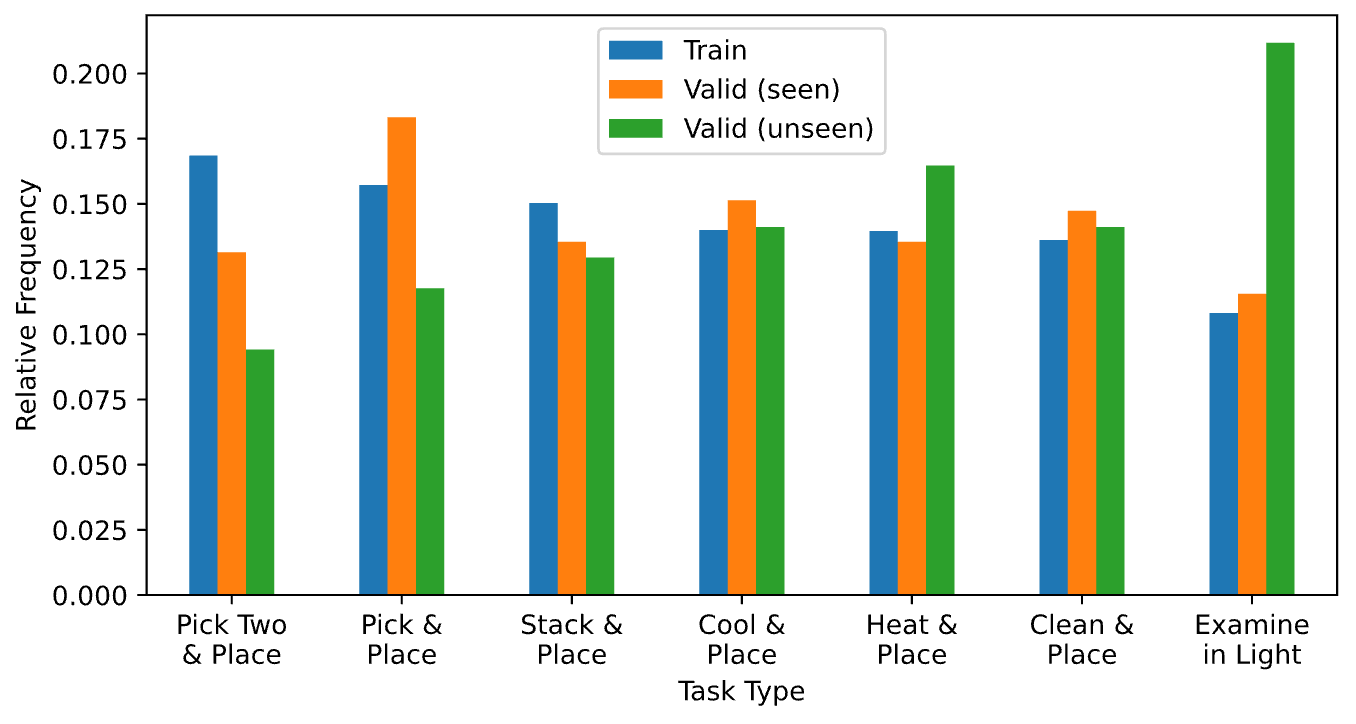
\includegraphics[scale=0.33]{figures/task_type_freqs.png}
\caption{Relative frequency of each task type by split}
\label{fig:task-type}
\end{figure}

\subsection{Hard to compute baselines/metrics}
\label{app:missed}
In the following, we list out all baselines/metrics that we planned to run, but could not due to reasons listed below.

\begin{itemize}
    \item \textbf{Seq-2-Seq (CNN-LSTM)} \cite{shridhar2020alfred} We did not evaluate the vanilla CNN-LSTM Seq2Seq architecture because a) we evaluated the progress monitoring variant that gets better performance, and b) the pre-trained model for this was not provided and we wanted to spend our limited compute on better performing models like MOCA \cite{singh2020moca}.
    \item \textbf{Modular Seq-2-Seq} \cite{corona2020modularity} We did not evaluate our internal metrics on the modular Seq2Seq architecture because their code was not released.
    \item \textbf{Seq-2-Seq RL (proposed):} Seq2Seq RL was an architecture we had originally proposed which basically used reinforcement learning to train the policy network which was same as the Seq2Seq PM architecture. However, we were not able to evaluate on this because of several reasons. One, we did some calculations on GPU compute and realized that training using RL would be very expensive which we would not be able to afford (at least not on models that we have not built). Two, we felt that the reward function would need to be heavily tuned to get any satisfactory performance, which would take a lot of time and probably not be considered a "baseline" model since we would have heavily modified it. Three, many libraries/implementations did not support recurrent policies which was just another challenge in implementing this.
    \item \textbf{Interaction Mask Prediction Performance (IMPP)}: We initially defined IMPP as the intersection over union score of the predicted instance segmentation mask with respect to the ground truth mask when the interaction action was correct. The idea was that conditioning on correctness of interaction action would make IMPP only measure the performance of the component that predicts the interaction mask. However, we could not compute this because there was no objective, non-heurestic based way to identify which object the agent intended to interact with at which time. Just matching expert action and predicted at each time step would be too naive because it is unlikely that the agent would mimic the expert so closely.
    \item \textbf{Length-conditioned Success (LCS)}: We initially wanted to compute LCS, which was supposed to be the first $n$ sub-goals successfully completed continuously. However, we could not compute this because the simulator does not store the ordering of the sub-goals, so we could not tell which sub-goals were first and which were last.
\end{itemize}

\subsection{Pipeline features}
\label{app:code}

\begin{enumerate}
    \item Our pipeline uses very strong software engineering and object oriented design principles and strongly decouples all different parts that are logically distinct. Such decoupling allows models in our pipeline to be run without relying on any preprocessing or external dependencies.
    \item Currently, our pipeline supports both the baseline Seq2Seq model and MOCA under a unified interface, which will not only help us compare our model with them, but also all future researchers working on ALFRED who want to compare their models to other SOTA models.
    \item We also have built a Gym style \cite{brockman2016openai} environment for ALFRED, making it amenable to be trained using reinforcement learning easily.
    \item A strong component in helping us keep our code very clean is our custom designed solution for configuration management, which keeps all configuration variables and utility functions separate from the main code, essentially helping us achieve disentanglement between logically separate parts.
\end{enumerate}

\subsection{Previous ALFRED Models}

Figures \ref{fig:alfred_model} and \ref{fig:moca_model} show previously proposed architectures.

\begin{figure*}
    \centering
    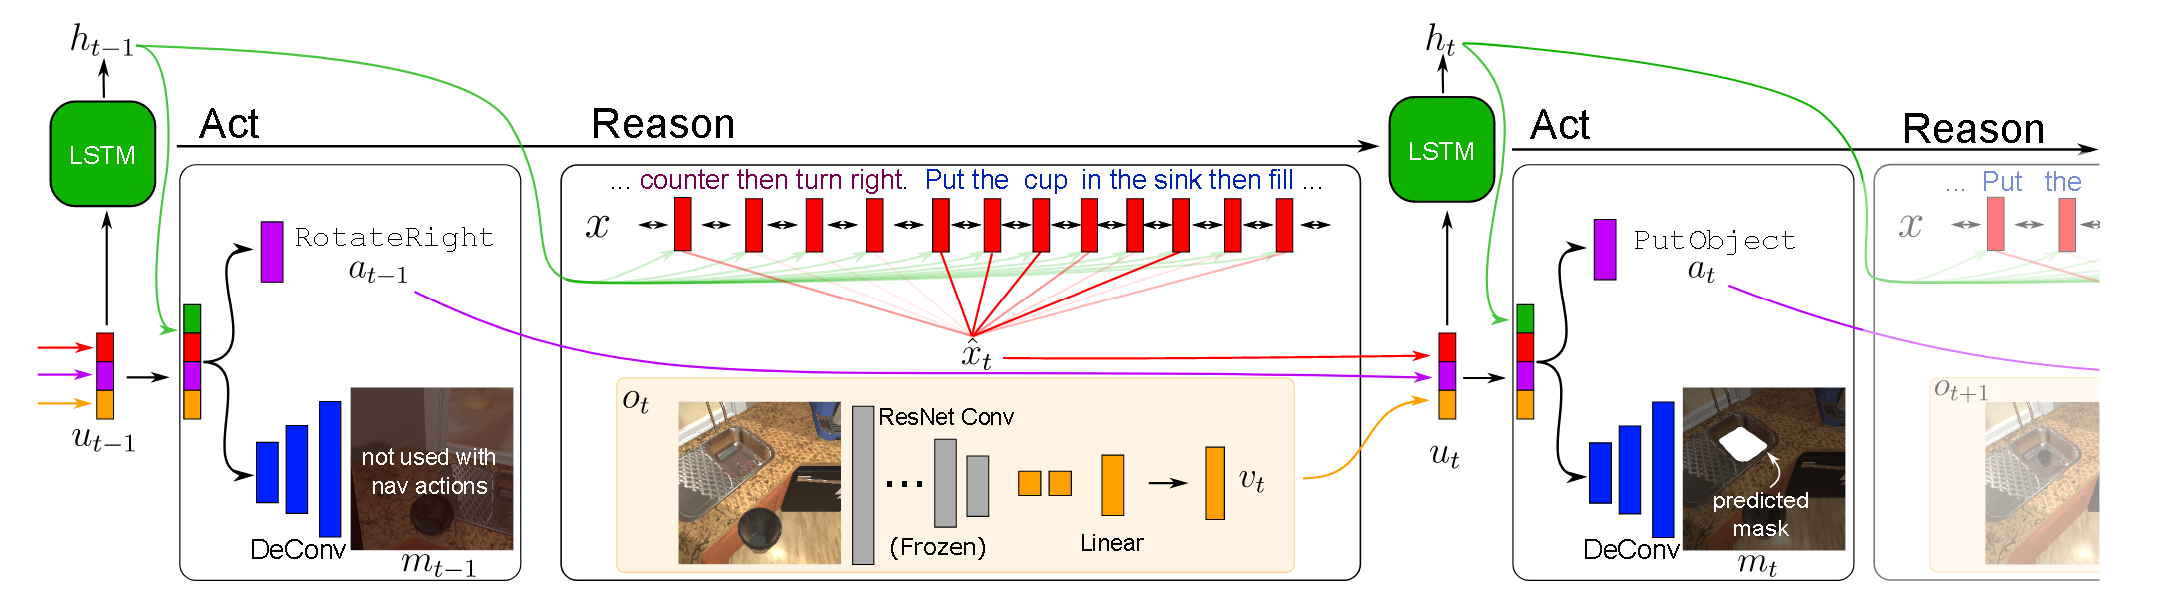
\includegraphics[scale=0.75]{figures/alfred_model.png}
    \caption{ALFRED Baseline Model \cite{shridhar2020alfred}}
    \label{fig:alfred_model}
\end{figure*}

\begin{figure*}
    \centering
    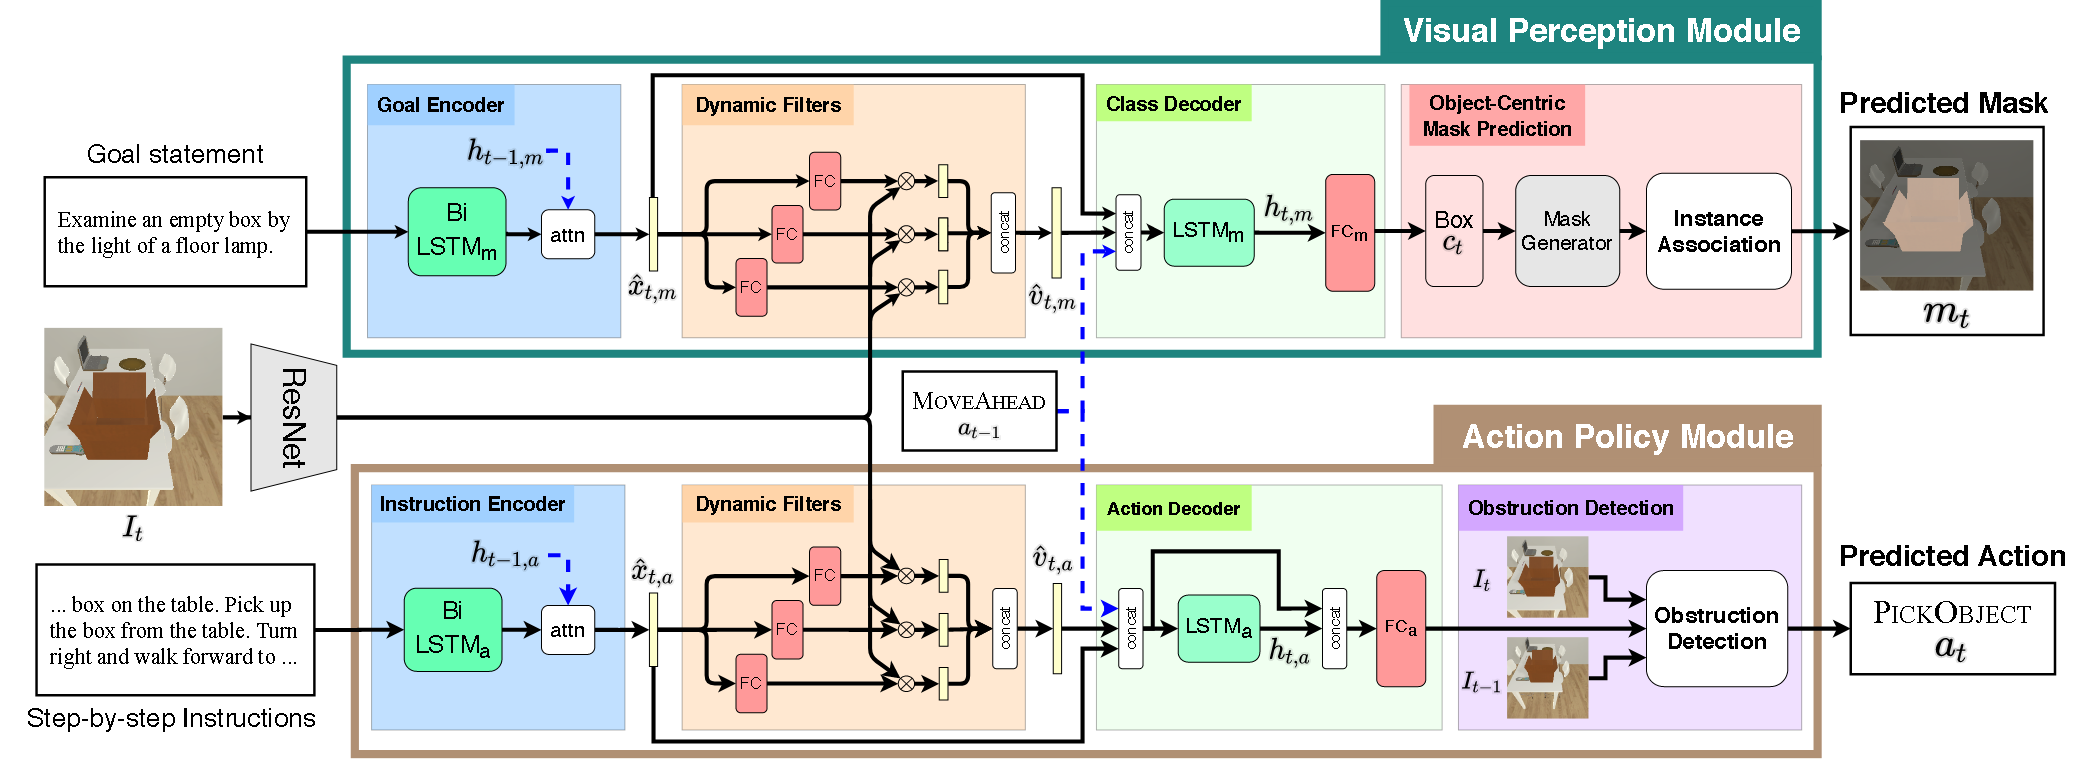
\includegraphics[scale=0.75]{figures/moca_model.png}
    \caption{MOCA Model \cite{singh2020moca}}
    \label{fig:moca_model}
\end{figure*}


\end{document}
